\section{Introduction}

The need to precisely quantify morphological variation in mycelial structures as a means of control in industrial fermentations has led to the deployment of computer-aided image processing as a tool for the study of microbial culture systems \cite{cox1998}. The detailed assessment of limited numbers of hyphal elements in both submerged \cite{spohr1998} and solid state systems \cite{bartnicki-garcia2000,dieguez-uribeondo2004} has contributed much to the understanding of apical growth mechanisms, while the derivation of average data from the monitoring of large cell populations \cite{carlsen1996a,spohr1997} is aimed at process optimization within bioreactor systems. Early progress in the development of automated routines \cite{tucker1992} led Thomas and Paul to declare in 1996 that \lq \emph{it is probable that fully automated image analysis will soon be used to gather the large amounts of data needed for both model extension and verification}' \cite{thomas1996}. However, many studies of morphology still rely on significant manual intervention \cite{mcintyre1997,wongwicharn1999,lubbehusen2003,rahardjo2005b,lecault2007}, which increases execution time and reduces throughput. There is therefore a pressing need for further development of automated image analysis systems for application in this field.

\subsection{Basic concepts of digital image processing}

The application of image analysis permits the translation of readily recognisable qualitative traits into actionable, quantitative data (Fig.~\ref{fig:AnalysisFlow}). The derivation of accurate data is dependent on the capture of representative images, as the integrity of the results will be compromised by low-quality input. The input process commences when the projection of a three-dimensional object is captured on a charge-coupled device (CCD) array, such as that contained within a digital camera or a flat-bed scanner, and is subsequently digitised. This digitisation causes the original two-dimensional, continuous, analogue representation of the image to be quantised at each point on the array, resulting in a digital representation of the field of view. The resolution (the number of pixels) of the resultant image is dependent on the size of the array on which the image was captured. Quantisation is generally performed uniformly, whereby the intensity at some point $(x,y)$ within the image is linearly translated to some integer value between $0$ and $2^M$, where $M$ is referred to as the bit depth of the resulting digital image. In most applications (and in most images used in this thesis) $M=8$, so each pixel is represented by an intensity value between 0 and 255 (Fig.~\ref{fig:Digitise}). Colour images generally have a bit-depth of 24, 8 bits for each colour component, red, green and blue.

\begin{figure}[htbp]
	\centering
	\pstool[width=(\textwidth - 1cm)]{../C2/AnalysisFlow}{
		\psfrag{o}[c]{\footnotesize Object}
		\psfrag{C}[c]{\footnotesize Image}
		\psfrag{c}[c]{\footnotesize Capture}
		\psfrag{P}[c]{\footnotesize Processing}
		\psfrag{p}[c]{\footnotesize of Image}
		\psfrag{d}[c]{\footnotesize Output Data}
		\psfrag{S}[c]{\footnotesize Control}
		\psfrag{s}[c]{\footnotesize System}
		\psfrag{H}[c]{\footnotesize Human}
		\psfrag{h}[c]{\footnotesize Observer}
		\psfrag{D}[c]{\footnotesize Data Storage}}
  \caption{Schematic representation of a typical image analysis system.}
  \label{fig:AnalysisFlow}
\end{figure}

\begin{figure}[htbp]
	\centering
	\subfloat{\label{fig:Quanta}\fbox{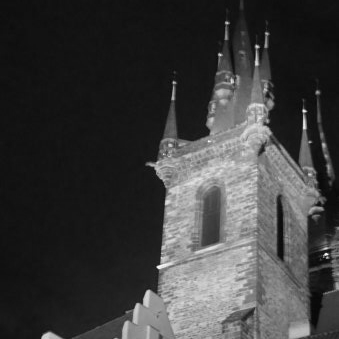
\includegraphics[height=6cm]{../C2/Quanta}}}
	\hspace{0.5cm}
	\subfloat{\label{fig:Quantb}\pstool[height=6cm]{../C2/Quantb}{
		\psfrag{x}[Bc]{\al $x$}
		\psfrag{y}[Bc]{\al $y$}
		\psfrag{255}[Bc]{\al\hspace{0.8cm} 255}}
	}
  \caption{Quantisation of intensity levels. Each $(x,y)$ coordinate in the image has an associated integer value between 0 and 255.}
  \label{fig:Digitise}
\end{figure}

Following image capture and digitisation, there are various forms of low- and high-level processing that may be performed. Roerdink categorised these as image pre-processing, segmentation, object description and finally, interpretation \cite{roerdink1998}. Pre-processing is based on the premise that the image contains both an object of interest and an added unwanted noise component, which may, for example, result from electrical disturbances in the CCD on which the image was captured. Other unwanted features that may require correction include non-uniform image background, poor image contrast or blurring. Once the image has been optimised, attempts are made to group together regions within the image based on some property, such as the intensity of the pixels. Image segmentation typically aims to separate objects of interest from the image background, but more generally, it is a means of identifying different regions. Common forms of segmentation are grey-level thresholding and edge detection and the result of segmentation is often the output of a binary image (Fig.~\ref{fig:Binarise}). Description then seeks to characterise the different regions identified by the segmentation stage using various properties: projected area, perimeter length, centre of mass, bounding rectangle, Feret's diameter, and radius of gyration, among others. Finally, it may be required that the various region descriptions be interpreted in some way, so as to, for example, eliminate a particular region from further analysis, or, to assign a particular classification to a region.

\begin{figure}[tb]
	\centering
	\fbox{
\includegraphics[height=6cm]{../C2/Bina}}
  \caption{Binary image of Figure~\ref{fig:Digitise}, in which only two grey levels are present.}
  \label{fig:Binarise}
\end{figure}

\subsection{Morphological classification of filamentous microbes}

A wide variety of parameters have been utilised in the study of microbial spores, hyphal elements, aggregates and pellets \cite{pons2000}, although many are derived from simple measures such as projected area ($\Ap$) or perimeter length ($P$). Means of identification of different structures have also received considerable attention and some of the different techniques utilised are outlined here.

\subsubsection{Analysis of spores}

Typical measures utilised in the analysis of spores include projected area and circularity ($C$), particularly in cases where the spores in question are approximately spherical \cite{spohr1998}. Teliospores and pycniospores of certain \emph{Puccinia} species are approximately ellipsoidal and have been quantified in terms of their major and minor axes \cite{anikster2005}. Other studies have utilised Fourier descriptors for more complex spore morphologies that cannot easily be described in terms of ellipsoids or spheres \cite{pazoti2005}.

Investigations into the influences on rates of spore germination have often relied on manual observation and counting to determine the percentage of germinated spores within a population \cite{pardo2005, sautour2001}. However, the use of a simple parameter such as circularity can prove useful in differentiating between germinated and non-germinated spores, as was demonstrated by Paul and colleagues \cite{paul1993}. The germinated spores were subsequently subjected to morphological filtering to separate the germ tube from the parent spore for analysis of each structure.  An automated method was also developed by Jones and colleagues, although the intended use was enumeration of spores in a haemocytometer for inoculum standardisation, rather than morphological quantification \cite{jones1992}.

\subsubsection{Enumeration and analysis of hyphae}

While the study of hyphal development has taken on several different forms, the challenges associated with the quantification of these structures may be resolved into three general approaches: high-magnification assessment of individual hyphae, quantification of mycelial \lq trees' or free mycelial elements and the identification and subsequent analysis of mycelial aggregates. Determination of measures such as the hyphal growth unit ($\hgu$; ratio of total hyphal length to number of hyphal tips) and hyphal width is generally not possible from the same image given the differences in scale\footnote{Generally 2 -- 3 orders of magnitude between hyphal width and mycelial width} and capture of images at different magnifications is typically required for this purpose \cite{larralde-corona1997,haack2006}.

% Bartnicki-Garcia should probably be mentioned in the general introduction

At the high-magnification level, Bartnicki-Garc\'{i}a and colleagues used computer enhanced video-microscopy to map the trajectory of cell surface markers in growing hyphae of \emph{Rhizoctonia solani} to determine the pattern of cell wall expansion during apical growth \cite{bartnicki-garcia2000}. McIntyre and colleagues estimated lengths of apical compartments in hyphae by determining the distance between the apex and first septum (apical compartment) and between subsequent septa of each hyphal element \cite{mcintyre2001}. Other studies have yielded information on sub-cellular hyphal details. For example, Pollack and colleagues measured the percentage of vacuolated area as the total vacuole size per total mycelium size \cite{pollack2008}. Vacuolation was also used to differentiate between active and non-active hyphal regions of \emph{A.~niger}, permitting estimations of the percentage of active biomass \cite{wongwicharn1999, wongwicharn1999a}.

Numerous studies of mycelial architectures have been reported, but one of the earlier systems was developed by Packer and Thomas, which permitted the determination of total hyphal length, main hyphal length (by determination of the longest connected path), hyphal branch length and hyphal growth unit in mycelial \lq trees' \cite{packer1990}. An estimation of the percentage of biomass occurring in clumped form was also included. This system was later enhanced to include a novel means of first identifying, then characterising, clump morphology in terms of projected area, circularity and convex perimeter ($P_c$; Fig.~\ref{fig:Fig4Tucker1992}) \cite{tucker1992}. Similar approaches to the quantification of mycelial trees and clumps have been employed in several other studies \cite{elsabbagh2006,mcintyre1998,amanullah2000,li2000}. Lecault and colleagues proposed an intermediate classification between free elements and clumps, termed an entangled mycelium, identified based on the number of \lq holes' in the structure \cite{lecault2007}. They also produced more extensive data on dispersed growth forms, including the mean, minimum and maximum branch lengths, as well as the mean, minimum, and maximum inter-nodal distances and the number of inter-nodal units. The branching order was determined by calculating the number of iterations required to subtract all of the end points, similar to the method described by Tucker and colleagues \cite{tucker1992}. Other studies have adopted a more general approach, measuring all biomass present in terms of projected area, as constant hyphal width implies area is proportional to biomass, so specific biomass fractions can be derived \cite{li2000,bhargava2003,bhargava2003a,bhargava2005}.

\begin{figure}[tb]
	\centering
	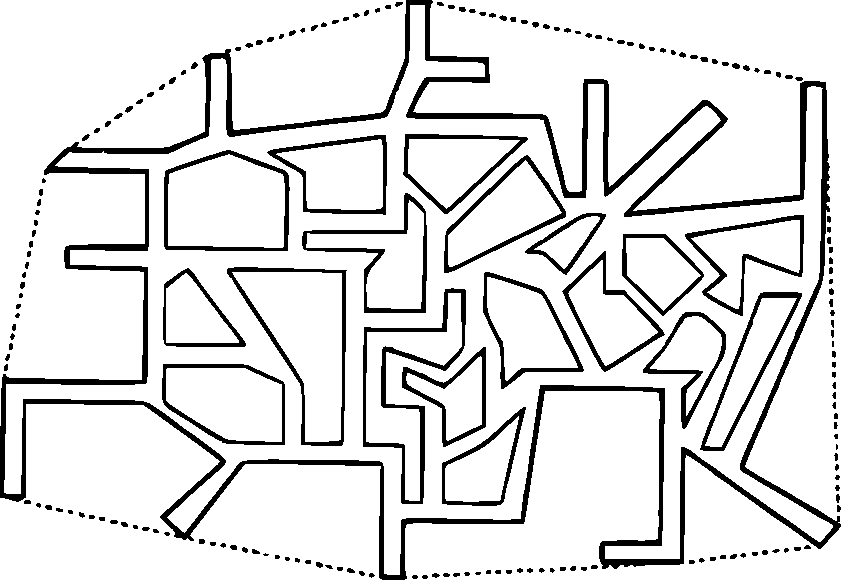
\includegraphics[width=8cm]{../C2/Fig4Tucker1992}
  \caption{A mycelial clump, as illustrated by Tucker and colleagues, with the convex perimeter ($\Pc$) indicated by the dotted line \cite{tucker1992}. Reproduced with permission from John Wiley and Sons.}
  \label{fig:Fig4Tucker1992}
\end{figure}

\subsubsection{Classification of dense aggregates and pellets}

Conventional measures of dense, pellet-like aggregates (Table~\ref{tab:MorphParam}) include projected area, equivalent diameter ($\Dp$), circularity, perimeter, projected convex area (area including holes; $A_c$) and convex perimeter \cite{cox1998}. Various other metrics have been employed, which generally involve some combination of the above, such as \lq roughness' \cite{higashiyama1999}, \lq compactness' \cite{muller2002,jppark2002,muller2003} and \lq convexity'  \cite{papagianni2002,papagianni2004}. Lucatero and colleagues used a combination of shape factors to distinguish between free hyphae, clumps and pellets \cite{lucatero2004}. Objects exhibiting a mean diameter of less than 0.3~mm were considered dispersed mycelia. Clumps were considered to be particles larger than 0.3~mm and of compactness (estimation of density) lower than 0.99, while pellets were defined as particles having a compactness between 0.99 -- 1 and roundness (deviation from a circle) less than 6. Similarly, a clump was defined by M\"{u}ller and colleagues as a structure with \mic{$\Dp >40$} and $\Ap/A_c > 0.55$ \cite{muller2002}.

\begin{table}[tb]
	\centering
	\footnotesize
	\caption{Some commonly used parameters in the morphological description of mycelial aggregates and pellets.}
	\label{tab:MorphParam}
	\begin{tabularx}{(\textwidth - 1cm)}{l c R}
		\toprule
		Parameter & Definition & Description \\ \midrule
		Projected Area & $\Ap$ & Number of pixels representing an object.\\
		Equivalent Diameter & $\Dp = 2\sqrt{\Ap / \pi}$ & Diameter of a circle with area equivalent to $\Ap$.\\
		Perimeter & $P$ & The pixel length of an object boundary.\\
		Circularity & $C= (4 \pi \Ap)/P^2$ & A measure of deviation from a circle.\\
		Roughness & $R=P^2/\Ap$ &\\
		Projected Convex Area & $A_c$ & Number of pixels representing an object, including any enclosed \lq holes'.\\
		Convex Perimeter & $P_c$ & Perimeter of an object with all concavities filled (Fig.~\ref{fig:Fig4Tucker1992}).\\
		Compactness & $M=\Ap / A_c$ &\\
		Convexity & $E=P / P_c$ &\\
		\bottomrule
	\end{tabularx}
\end{table}

The mean grey-level intensity of regions has been utilised as an effective means of discriminating between dense aggregates, such as pellets, and less compact structures, such as mycelial aggregates or clumps \cite{papagianni2002,teng2009}. Similarly, a difference in grey levels between pellet core and periphery has been employed to distinguish between the two regions and derive separate measures of each \cite{cui1998b,truong2004}. Subsequent quantification of the pellet cores is thus possible, based on, for example, the ratio of the minimum Feret's diameter to the maximum \cite{hwang2004, jppark2002}. Others have operated on binary images with morphological filters to \lq erode' the annular region in both pellets \cite{koike2001,eypark2001} and clumps \cite{lucumi2005}, producing binary representations of aggregate cores. For example, Rodr\'{i}guez-Porcel and colleagues expressed pellet morphology as a ratio between the filamentous area and the total pellet area \cite{rodriguezporcel2005}, while Papagianni and Moo-Young included measures of the average length of the filaments that protruded from the core of clumps in their characterisation of \emph{A.~niger} \cite{papagianni2002}.

\subsubsection{Other macroscopic analyses}

Macroscopic and low-magnification microscopic analysis of mycelial growth on solid substrates has generally been restricted to measures of hyphal coverage or projected area of biomass \cite{couri2006,cross2004}. However, a significantly more detailed system was developed by D\"{o}rge and colleagues for the identification of different species of \emph{Penicillium}, based on colony colour distribution, colony dimensions and texture measurements \cite{dorge2000}. Image processing was also utilised in the evaluation of dye biotransformation by the white rot fungi \emph{Pycnoporus cinnabarinus} and \emph{Phanerochaete chrysosporium} \cite{jones1993b}.

\subsection{Development platform}

ImageJ is a public domain, Java image processing program designed with an open architecture that provides extensibility via Java plug-ins \cite{imagej}. It comes pre-equipped with many standard image processing capabilities, such as image segmentation (thresholding, edge detection), various linear and non-linear filter implementations, frequency-domain operations and limited object classification and measurement. The ImageJ platform has previously been utilised in the study of filamentous micro-organisms \cite{papagianni2006b,rahardjo2005b,tebiesebeke2005}. 

\subsection{Aims of the work in this chapter}

Extensive work on the classification of filamentous microbial morphology using digital image processing is evident in the literature, but fully automated systems are still rare. A wide range of approaches have been adopted during the course of these studies, but many studies have been specific to the analysis of one particular growth form or used a limited number of morphological parameters.

The aim of this chapter was to develop an integrated application, based on the ImageJ platform, that may be used as a means of quantifying any form of filamentous fungal morphology. The programme would proceed automatically and generate data on the population of spores, mycelia or pellets analysed and output this data to the user. In the design of this system, speed-of-execution was prioritised to provide a system capable of near-real-time analysis.

The design drew on many established methods in digital image analysis, for image pre-processing in particular, which were deemed suitable for this application. A survey of some popular pre-processing techniques was conducted and the most appropriate for this application selected. The morphological parameters incorporated into the design were based largely on the review of the literature. However, a more extensive quantification of hyphal elements in particular was targeted, so as to permit the compilation of data beyond the conventional hyphal growth unit and provide more detailed information on the branching strategies of filamentous micro-organisms.